\documentclass[12pt]{article}

% Use English with babel.
\usepackage[english]{babel}
% Use T1 font encoding. This should be imported before inputenc.
\usepackage[T1]{fontenc}
% UTF-8 character encoding.
\usepackage[utf8]{inputenc}
% Use the float package, for float option H.
\usepackage{float}
% Use math symbols.
\usepackage{amssymb}
\usepackage{amsmath}
% See: https://tex.stackexchange.com/a/166127
\usepackage{textcomp}
% Use more text and math symbols.
\usepackage{gensymb}
% Use SI units and scientific notation.
\usepackage{siunitx}
% Use url. This is necessary to have links with sectional URLS. https://tex.stackexchange.com/a/547221
\usepackage{url}
% Use listings, for source code formatting.
\usepackage{listings}
\lstset{
  language=Python,
  aboveskip=3mm,
  belowskip=3mm,
  showstringspaces=false,
  columns=flexible,
  basicstyle={\small\ttfamily},
  numbers=none,
  numberstyle=\tiny\color{gray},
  keywordstyle=\color{blue},
  commentstyle=\color{dkgreen},
  stringstyle=\color{mauve},
  breaklines=true,
  breakatwhitespace=true,
  tabsize=2
}
% Use natbib, for URLs in the bibliography.
\usepackage{natbib}
% See: https://tex.stackexchange.com/a/10928.
\usepackage{etoolbox}
\apptocmd{\sloppy}{\hbadness 10000\relax}{}{}
% Use graphics.
\usepackage{graphicx}
\graphicspath{ {../data/calc_current_1/} {../data/calc_current_2/} {../data/time_v_current_base/} {../data/time_v_current_vary_density/} {../data/time_v_current_vary_lifetime/} }
% Use hyperlinks. This should be imported last.
\usepackage{hyperref}
\hypersetup{
    colorlinks=true,
    linkcolor=blue,
    filecolor=magenta,
    urlcolor=cyan,
    citecolor=blue
}


\title{Photoconductor Research}
\author{Kyle Loerker}
\date{\today}

\begin{document}

\maketitle

\section{Calculating electrical current}

We understand that intrinsic semiconductors do not conduct much electricity if any. Extrinsic semiconductors do conduct electricity, with their added amount of charge carriers. Given a uniform electric field and density, resistance can be represented by \citep{wikipedia_resistivity_ideal}:
\begin{equation}
  R=\rho\frac{\ell}{A} \label{eq:resistance}
\end{equation}
In our simulation of a thin slab of silicon, we may apply this equation as the density and doping of the material is uniform, and the electric field is constant, as seen in figure \ref{fig:efield}.

For a doped semiconductor, there are a couple of ways of determining the electrical resistivity $\rho$:
\begin{itemize}
  \item Finding the resistivity of the doped material as a function of the amount of electrons and/or electron holes, with this equation \citep{colorado_resistivity} \citep{wikipedia_resistivity}:
        \begin{equation}
          \sigma=q(\mu_nn+\mu_pp) \label{eq:conductivity}
        \end{equation}
        $q$ is the charge, where $q=e=\SI{1.60e-19}{C}$. $n$ is the number of electrons, and $p$ is the number of electron holes. $\mu_n$ and $\mu_p$ are the mobilities of the electrons and holes, respectively. When there is a negligible amount of minority carriers, this equation can be simplified to $\sigma=q\mu_nn$ or $\sigma=q\mu_pp$. Finally, $\rho$ is the reciprocol of electrical conductivity $\sigma$.
  \item Finding the resistivity at a single point, with the equation $\rho=\frac{E}{L}$. $E$ is the magnitude of the electric field, and $J$ is the magnitude of the current density, at this point. This is a more general equation, but it can be useful for us as $E$ and $J$ are constant throughout our chip.
\end{itemize}

\begin{figure}[H]
  \centering
  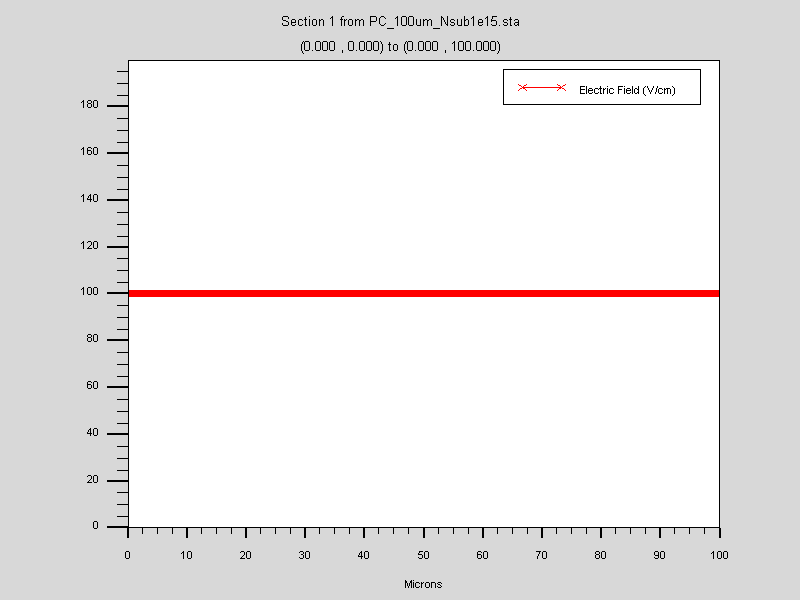
\includegraphics[width=\textwidth]{efield}
  \caption{Graph of the magnitude of the electric field across the chip.}
  \label{fig:efield}
\end{figure}

Unless specified otherwise, the following examples will assume the following:
\begin{itemize}
  \item $N_d=\SI{1e15}{cm^{-3}}$.
  \item The substrate material is silicon, and the dopant material is phosphorus.
  \item The temperature is $300{\degree}K$.
\end{itemize}

\subsection{Using a calculator}
\href{https://www.pvlighthouse.com.au/resistivity}{This} online calculator can be used to determine what the resistivity of a given doped semiconductor will be, taking dopant concentration $N_d$ as an input. According to this calculator, $\rho=4.584{\Omega}cm$.

\subsection{Using a graph}
Similarly to the last method, one can also use a graph of $N_d$ vs. $\rho$ to determine resistivity, such as that of \href{https://www.quora.com/What-is-the-effect-of-doping-on-resistance}{this} Quora answer. According to this group, $\rho\approx5{\Omega}cm$.

\subsection{Calculating from E-field and current density}
Using Silvaco TCAD, it can be found that $E=100.\frac{V}{cm}$ and $J=21.9\frac{A}{cm^2}$ (see figure \ref{fig:efieldcurrentdensity}), which can be used to find the resistivity:
\begin{equation}
  \rho=\frac{E}{L}=\frac{100.\frac{V}{cm}}{21.9\frac{A}{cm^2}}=4.564{\Omega}cm
\end{equation}
\begin{figure}[H]
  \centering
  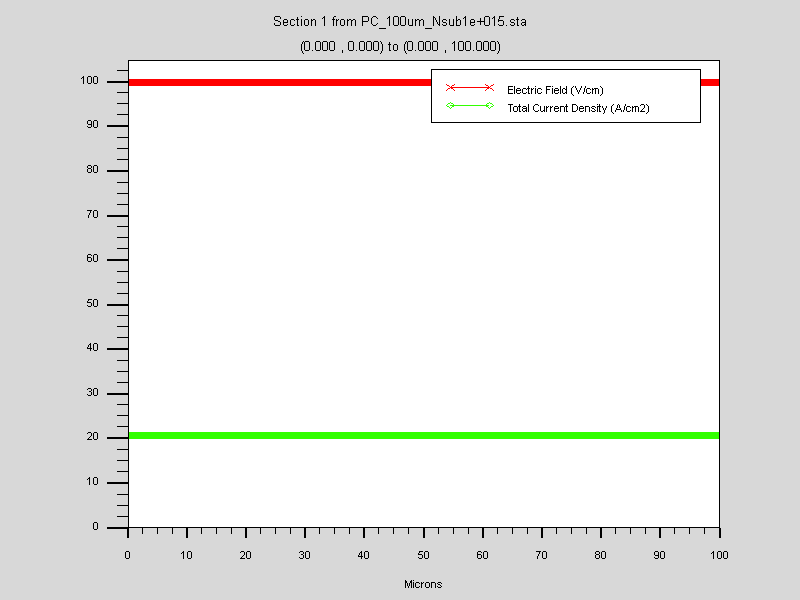
\includegraphics[width=\textwidth]{efieldcurrentdensity}
  \caption{Magnitude of the electric field and current density across the chip.}
  \label{fig:efieldcurrentdensity}
\end{figure}

\subsection{Calculating from doping concentration}
$\mu_n$ is tricky to determine by hand, as it is related to the drift velocity \citep{wikipedia_mobility}. I have used the calculator from before to determine that $\mu_n=1324\frac{cm^2}{Vs}$. The calculator takes electron and hole lifetimes as a parameter, which we can extract from the \lstinline{material} parameter of the deck:
\begin{lstlisting}
  material region=1 taun0=1e-7 taup0=1e-7
\end{lstlisting}
These parameters do not seem to affect the mobilities anyways, though. The concentration of electrons can be found using TCAD (see figure \ref{fig:econc}), $n=\SI{1e15}{cm^{-3}}$ (equivalent to our doping concentration). These can be used to find the resistivity:
\begin{equation}
  \rho=\frac{1}{q\mu_nn}=\frac{1}{(\SI{1.60e-19}{C})(1324\frac{cm^2}{Vs})(\SI{1e15}{cm^{-3}})}=4.54{\Omega}m
\end{equation}

\begin{figure}[H]
  \centering
  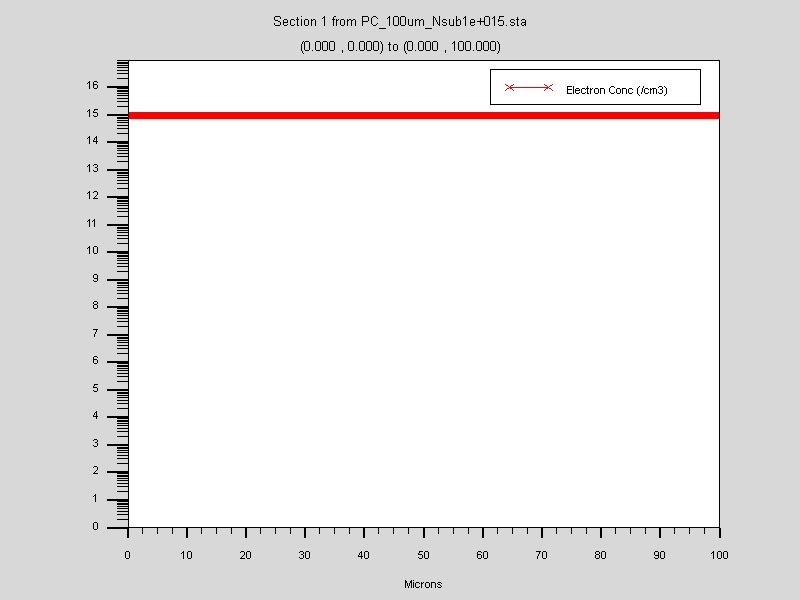
\includegraphics[width=\textwidth]{econc}
  \caption{Electron concentration across the chip.}
  \label{fig:econc}
\end{figure}

\section{Effect of dopant concentration and voltage on current}
Electrical current varies with the dopant type, dopant concentration, and voltage applied. The data from these experiments is available \href{https://docs.google.com/spreadsheets/d/1gYwgjLNNKRn5CSeJdrwOt3nx-jSYUwJLR_BUbzWCe9E/edit?usp=sharing}{here}. Figure \ref{fig:concvcurrent} shows the relationship between dopant concentration, and current. This graph includes the simulated current from the TCAD log files, and the current calculated using equations \eqref{eq:conductivity} and \eqref{eq:resistance}, where $I=\frac{V}{R}$. As $N_d$ increases, current {{I}} increases. For phosphorus, the simulated currents are lower, but for boron, the simulated currents are higher, when compared to their calculated counterparts.

\begin{figure}[H]
  \centering
  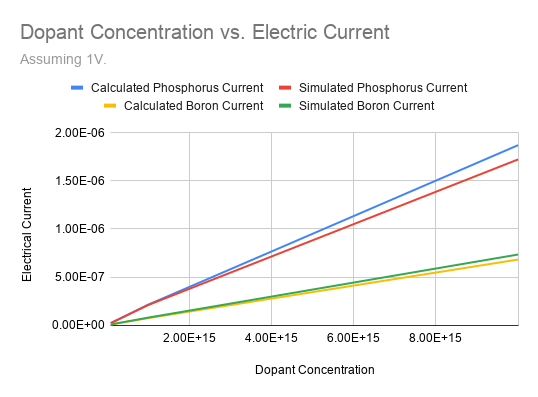
\includegraphics[width=0.5\textwidth]{concvcurrent}
  \caption{Electron concentration vs. dopant concentration for phosphorus and boron.}
  \label{fig:concvcurrent}
\end{figure}

Figure \ref{fig:voltvcurrent} shows the relationship between voltage, and current. As expected, larger voltages yield larger currents; it is worth noting that the deficit was much larger with phosphorus than with boron.

\begin{figure}[H]
  \centering
  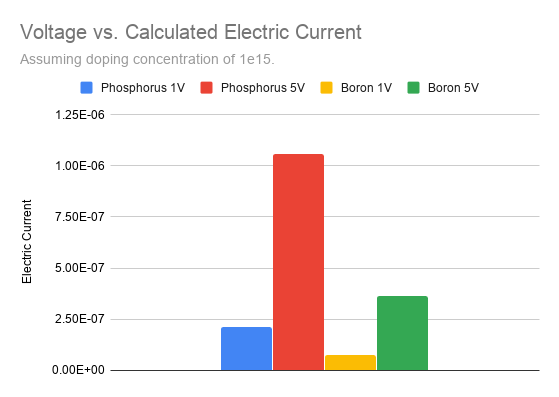
\includegraphics[width=0.5\textwidth]{voltvcurrent}
  \caption{Dopant concentration for phosphorus and boron at different voltages.}
  \label{fig:voltvcurrent}
\end{figure}

\section{Change in current over time}
To study the change in current flowing through the chip, the single-event upset was modified from it's original behavior of moving from $(50, 10)$ to $(60, 10)$, to moving from $(0, 50)$ to $(1, 50)$. Additionally, the density was changed from $\SI{1.14e-4}{\frac{pC}{{\mu}m}}$ to $\SI{1.0e-4}{\frac{pC}{{\mu}m}}$.

We have already logged the current flowing through the chip for different applied voltages. As can be seen in figure \ref{fig:voltvcurrentlog}, $V$ and $I$ are proportional, which makes sense as the two electrodes are configured to be ohmic. Now, we will study the current flowing through the chip for different times after the single-event upset.

\begin{figure}[H]
  \centering
  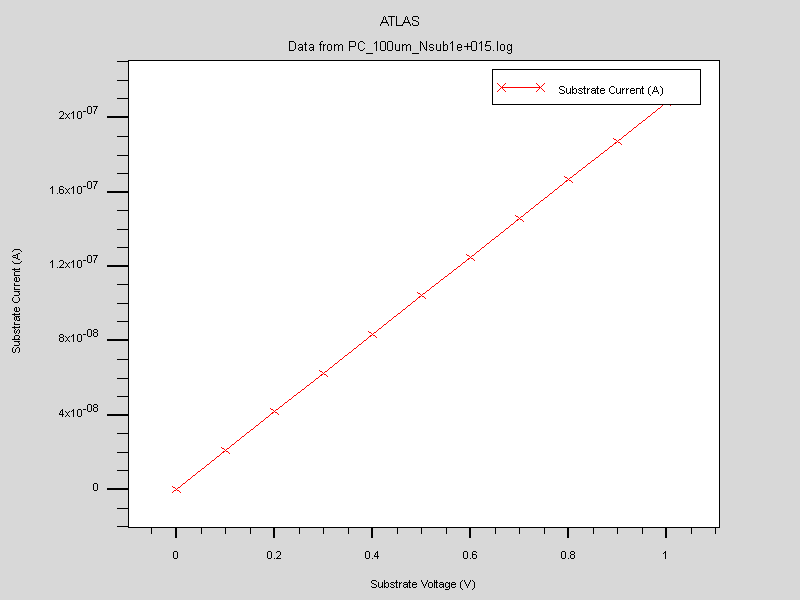
\includegraphics[width=\textwidth]{voltvcurrentlog}
  \caption{Substrate voltage vs substrate current.}
  \label{fig:voltvcurrentlog}
\end{figure}

In order to study this change, three variables were modified:
\begin{itemize}
  \item \lstinline{dt.max}, the maximum time-step for the transient simulation to run to. Transient simulations allow one to study the changed caused by an event like a sudden charged particle, and how the electronics react. This is opposed to studying electronics in their stable condition, without these upsets \citep{deshpande}.
  \item \lstinline{dt}/\lstinline{tstep}, the time-step to start at.
  \item \lstinline{tfinal}, the time-step to end at.
\end{itemize}
All three of these variables were increased by an order of magnitude each time.

The current gradually decreases over time. It decreases linearly at first, before the rate starts to lessen at about $\SI{1e-7}{s}$.

\begin{figure}[H]
  \centering
  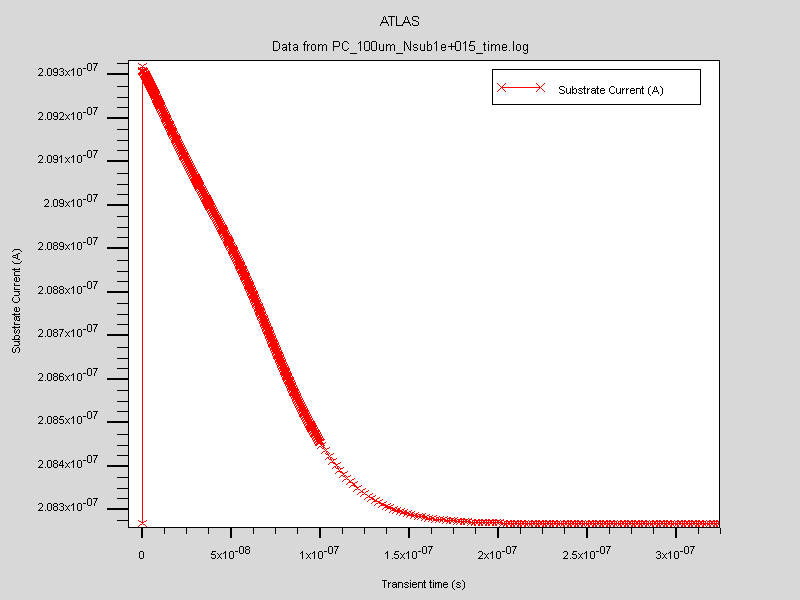
\includegraphics[width=0.5\textwidth]{timevcurrent}
  \caption{Time vs substrate current.}
\end{figure}

In the initial simulations of specific time-stamps depicted in figure \ref{fig:distancevcurrent}, it can be seen that a change in the electric field is propagated. By $\SI{1e-6}{s}$, the electric field seems to become constant once more.

\begin{figure}[htp]
  \centering
  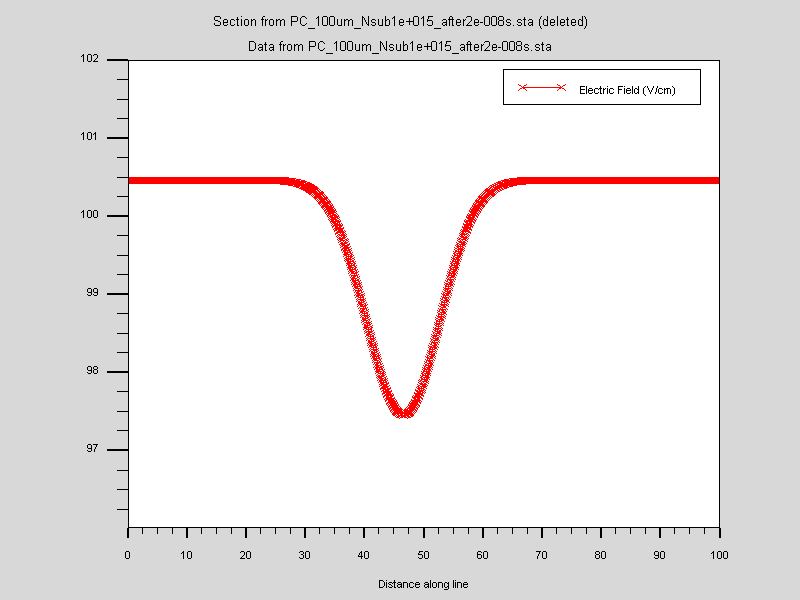
\includegraphics[width=.3\textwidth]{PC_100um_Nsub1e+015_after2e-008s}\hfill
  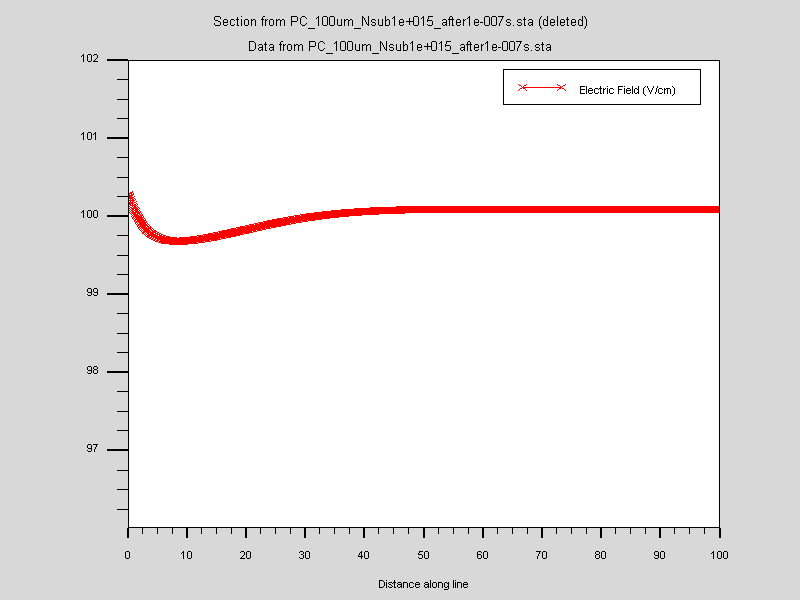
\includegraphics[width=.3\textwidth]{PC_100um_Nsub1e+015_after1e-007s}\hfill
  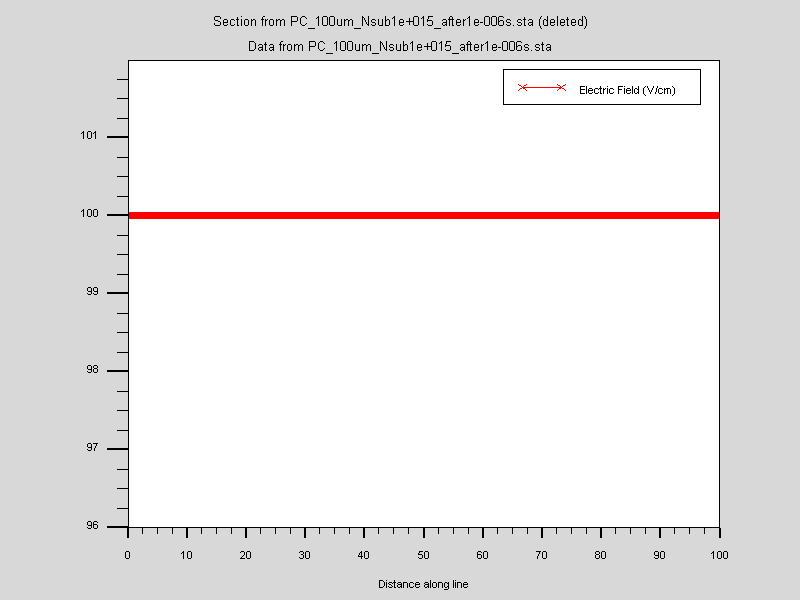
\includegraphics[width=.3\textwidth]{PC_100um_Nsub1e+015_after1e-006s}
  \caption{Distance vs substrate current after $\SI{20}{ns}$, $\SI{1e-7}{s}$, and $\SI{1e-6}{s}$.}
  \label{fig:distancevcurrent}
\end{figure}

\subsection{Modifying electron-hole pair density}

% Break this line to prevent an overful hbox.
To further study this, the density of electron-hole pairs present in the single-event upset was changed from it's default of $\SI{1.0e-4}{\frac{pC}{{\mu}m}}$ , from \\$\SI{1.0e-2}{\frac{pC}{{\mu}m}}$ to $\SI{1.0e-5}{\frac{pC}{{\mu}m}}$. According to figure \ref{fig:distancevcurrent_density}, greater densities yield greater electron and hole concentrations. Fluctuations in electron holes are greater than that of electrons. This data seems to confirm that the event is finished at $\SI{1e-6}{s}$.

  % It seems to me that, because of the way we broke up that last paragraph, the rest of this section becomes annoying. Weird and annoying, but eh.
  \begin{figure}[htp]
    \centering
    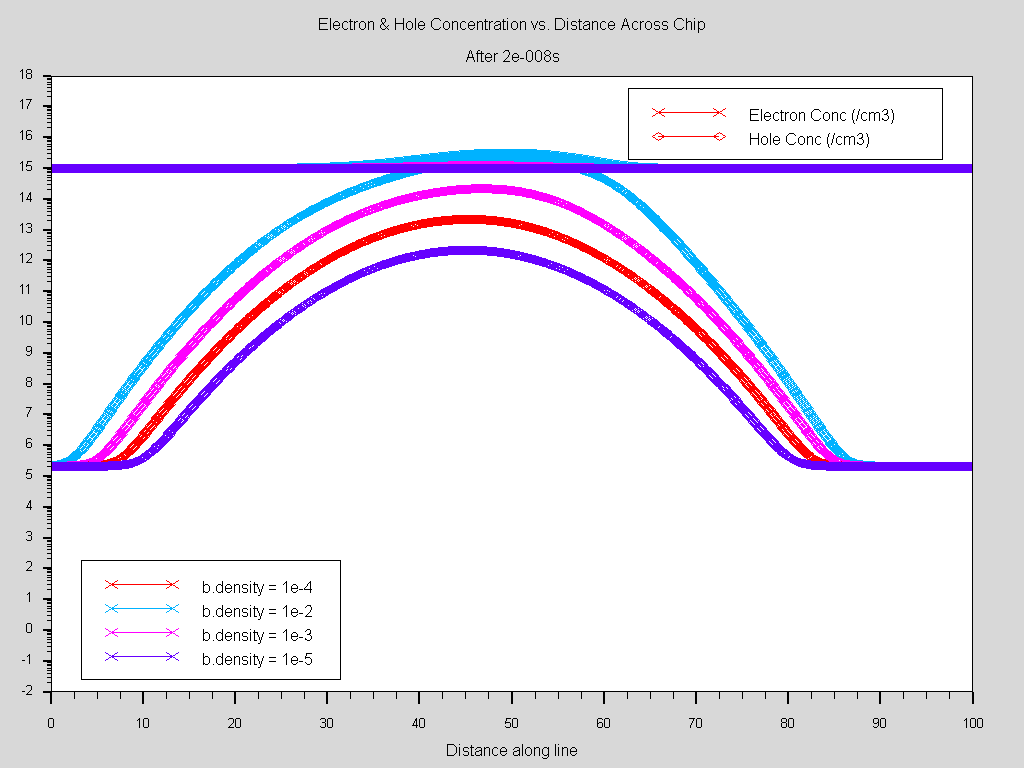
\includegraphics[width=.3\textwidth]{density_after2e-008s}\hfill
    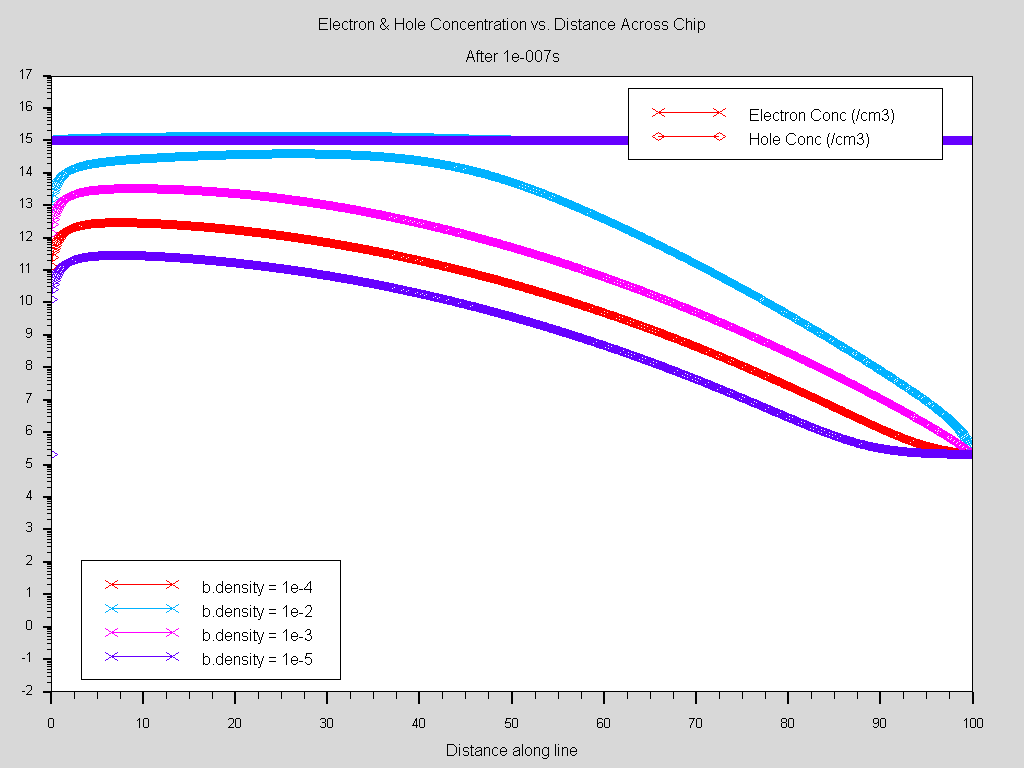
\includegraphics[width=.3\textwidth]{density_after1e-007s}\hfill
    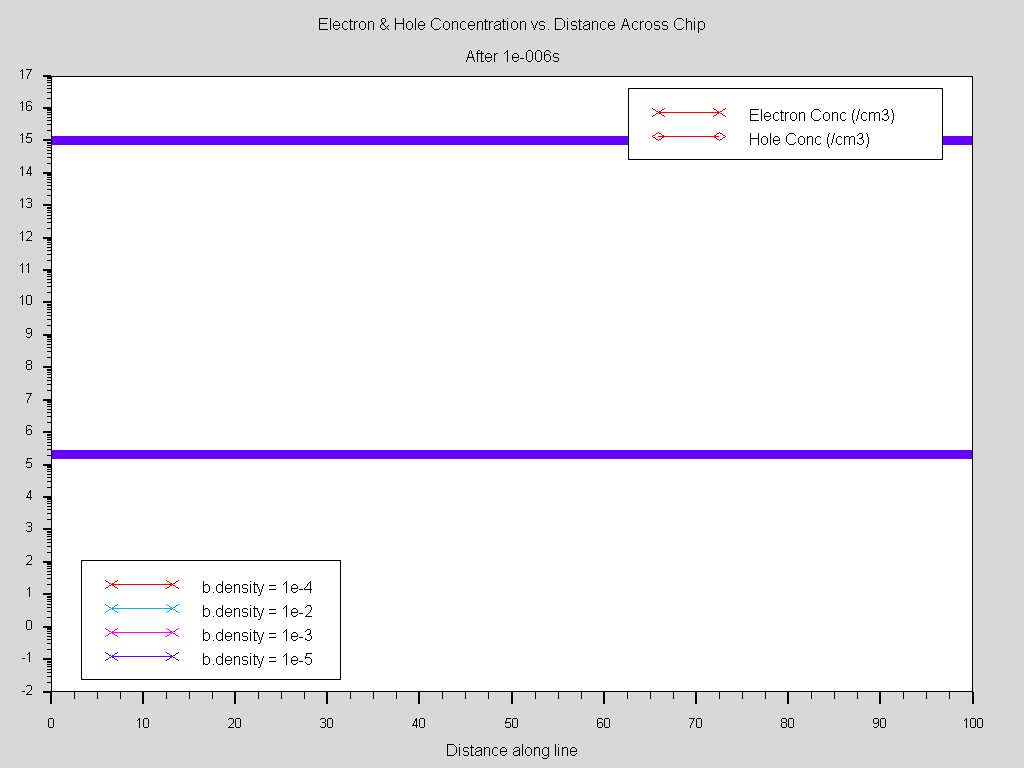
\includegraphics[width=.3\textwidth]{density_after1e-006s}
    \caption{Distance vs $e^-$/$h^+$ concentraion after $\SI{20}{ns}$, $\SI{1e-7}{s}$, and $\SI{1e-6}{s}$.}
    \label{fig:distancevcurrent_density}
  \end{figure}

  \subsection{Modifying electron-hole pair lifetimes}

  The parameters for the lifetimes for the electrons and holes were changed from $\SI{1e-7}{s}$, from $\SI{1e-6}{s}$ to $\SI{1e-8}{s}$.

\begin{figure}[htp]
  \centering
  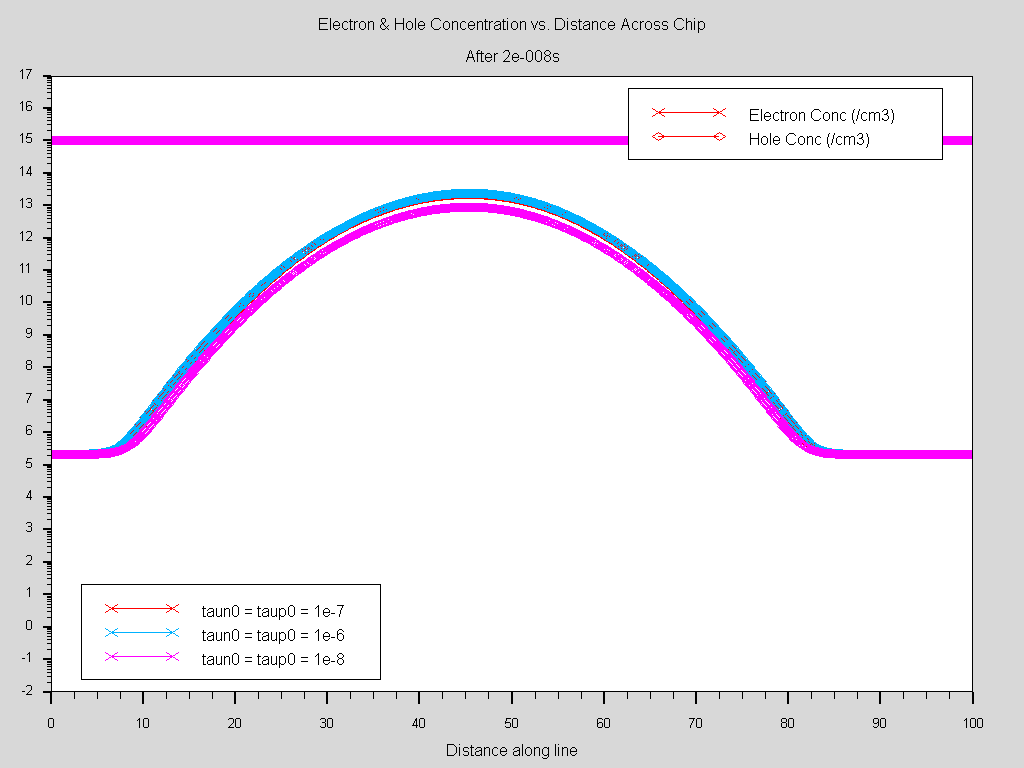
\includegraphics[width=.3\textwidth]{lifetime_after2e-008s}\hfill
  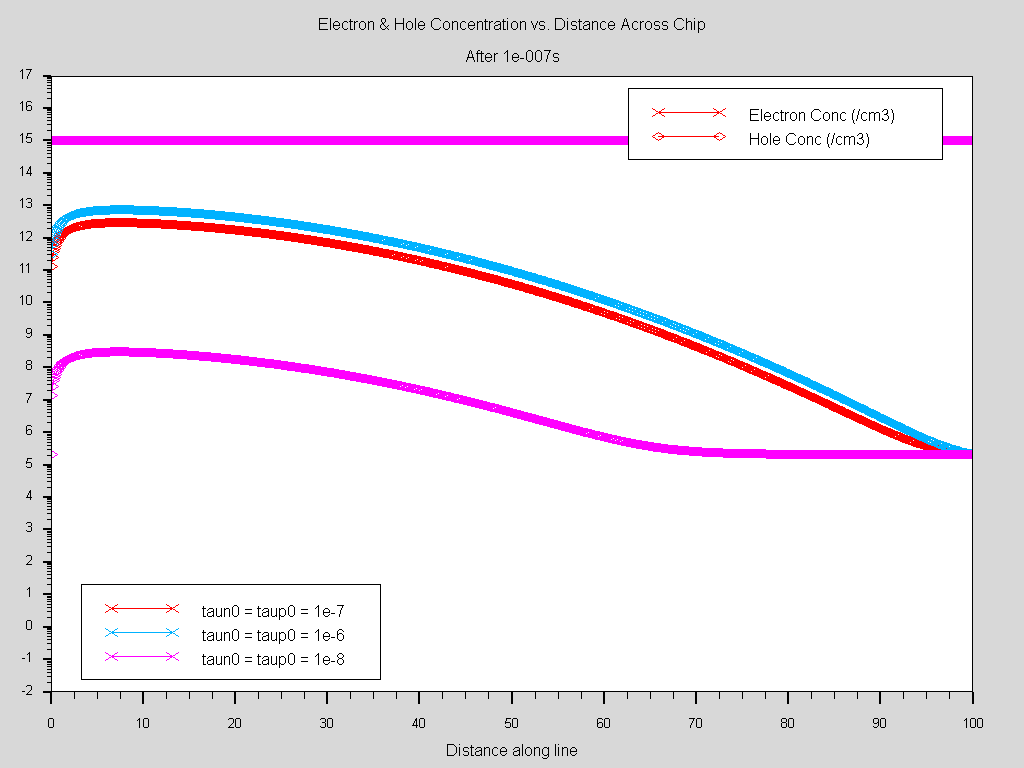
\includegraphics[width=.3\textwidth]{lifetime_after1e-007s}\hfill
  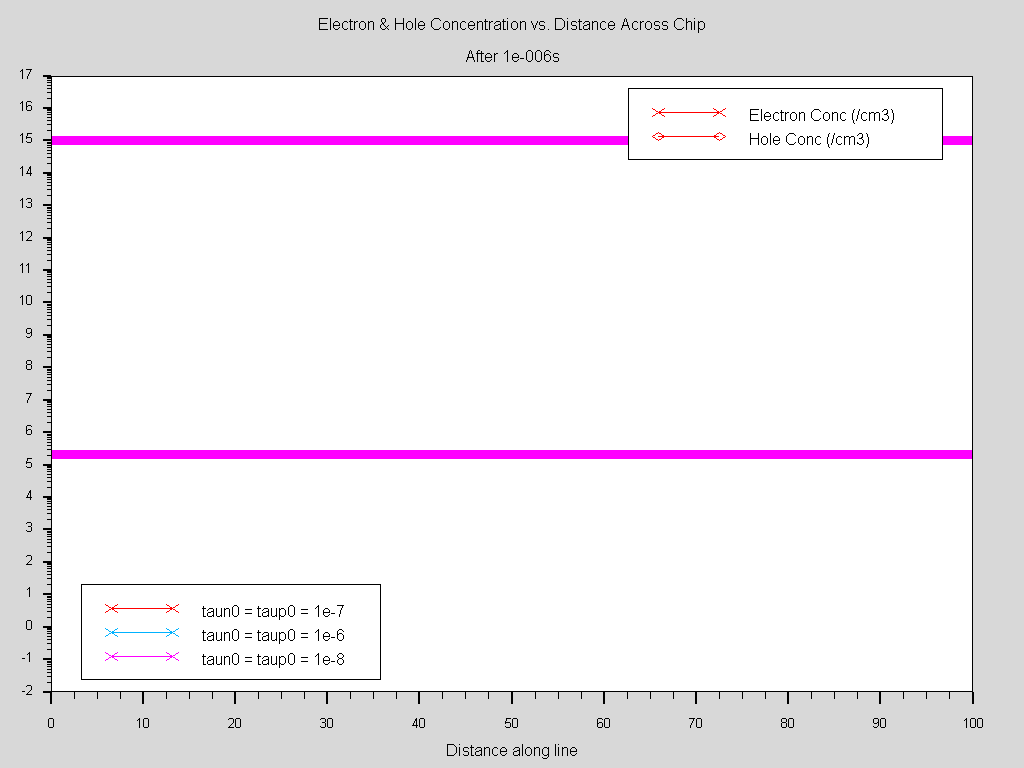
\includegraphics[width=.3\textwidth]{lifetime_after1e-006s}
  \caption{Distance vs $e^-$/$h^+$ concentraion after $\SI{20}{ns}$, $\SI{1e-7}{s}$, and $\SI{1e-6}{s}$.}
  \label{fig:distancevcurrent_lifetime}
\end{figure}

\bibliography{Experiments}
\bibliographystyle{unsrtnat}

\end{document}
